\documentclass[aspectratio=169]{beamer}
\usetheme{Madrid}
\usecolortheme{default}
\usepackage{tikz}
\usetikzlibrary{calc,shapes,arrows.meta,positioning}

% --- Organization slides (TOC + section dividers) ---
\AtBeginSection[]
{
  \begin{frame}{Outline}
    \tableofcontents[currentsection]
  \end{frame}
}

\title{Lecture 4: AI Agents \& Tool Use}
\subtitle{Building an Application Routing Agent}
\author{University of Chicago}
\date{\today}

\begin{document}

\frame{\titlepage}

% Global outline
\begin{frame}{Outline}
  \tableofcontents
\end{frame}

\section{Review and Context}

\begin{frame}{What We've Covered So Far}
\textbf{Lecture 1: Foundations}
\begin{itemize}
    \item Understanding LLMs, tokens, context windows, and APIs
    \item Token economics and pricing
\end{itemize}
\vspace{0.3cm}

\textbf{Lecture 2: Building AI Systems}
\begin{itemize}
    \item Vertical slices, Crawl-Walk-Run methodology
    \item Building a resume scoring system
\end{itemize}
\vspace{0.3cm}

\textbf{Lecture 3: Improving Performance}
\begin{itemize}
    \item Decomposition, grounding with citations, few-shot examples
    \item Improving the resume scorer
\end{itemize}
\end{frame}

\begin{frame}{Limitations We've Encountered}
\textbf{Our current systems are limited to text input and text output}:
\begin{itemize}
    \item LLMs can only process text and generate text
    \item They cannot directly:
    \begin{itemize}
        \item Query databases or retrieve external information
        \item Call APIs or interact with web services
        \item Schedule meetings or send emails
        \item Make decisions that trigger multiple sequential actions
    \end{itemize}
    \item Each call is independent - no persistence or state management
\end{itemize}
\vspace{0.3cm}

\textbf{Today}: Learn how to give LLMs the ability to interact with the world through \textbf{tools} and \textbf{agentic systems}
\end{frame}

\section{AI Agents}

\begin{frame}{What is an AI Agent?}
\begin{itemize}
    \item An \textbf{AI Agent} is an LLM that can use \textbf{tools} to interact with the outside world
    \item While a basic LLM can only generate text based on its training data, an agent can interact with ``tools" that:
\begin{itemize}
    \item \textbf{Database Tools}: Query databases, insert/update/delete records
    \item \textbf{API Tools}: Call REST APIs, interact with web services
    \item \textbf{File System Tools}: Read/write files, list directories
    \item \textbf{Code Execution Tools}: Run Python code, execute shell commands
    \item \textbf{Web Tools}: Search the web, scrape websites
    \item ...and more
\end{itemize}
\end{itemize}
\end{frame}


\begin{frame}{How Do They Work?}
\textbf{Agents are surprisingly simple}:
\vspace{0.3cm}

\begin{center}
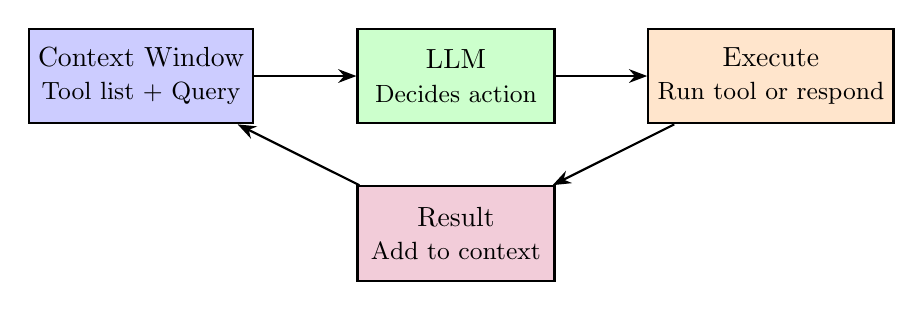
\begin{tikzpicture}[
  box/.style={rectangle, draw, thick, minimum width=2.5cm, minimum height=1.2cm, text centered, align=center},
  arrow/.style={->, thick, >=Stealth}
]
  \node[box, fill=blue!20] (context) at (0,0) {Context Window \\ {\small Tool list + Query}};
  \node[box, fill=green!20] (llm) at (4,0) {LLM \\ {\small Decides action}};
  \node[box, fill=orange!20] (execute) at (8,0) {Execute \\ {\small Run tool or respond}};
  \node[box, fill=purple!20] (result) at (4,-2) {Result \\ {\small Add to context}};

  \draw[arrow] (context) -- (llm);
  \draw[arrow] (llm) -- (execute);
  \draw[arrow] (execute) -- (result);
  \draw[arrow] (result) -- (context);
\end{tikzpicture}
\end{center}
\vspace{0.3cm}

\textbf{Key idea}: The LLM chooses which tool to use (or decides not to use any)
\end{frame}

\begin{frame}{The Agent Loop}
\begin{center}
We can simplify this into ``The Agent Loop"
\vspace{0.5cm}

\Large
Observe $\rightarrow$ Think $\rightarrow$ Act $\rightarrow$ Observe $\rightarrow$ \ldots
\end{center}
\vspace{0.8cm}
\begin{enumerate}
    \item \textbf{Observe}: Receive input (user query, tool results, system state)
    \item \textbf{Think}: Process information and decide what to do next
    \item \textbf{Act}: Execute actions (call tools, generate responses)
\end{enumerate}
\vspace{0.3cm}

\textbf{Each turn of the loop}:
\begin{enumerate}
    \item Agent sees: current state + what's been done so far
    \item Agent decides: which tool to call next (via LLM)
    \item Execute tool, log result
    \item Repeat until agent calls 'done' or max turns reached
\end{enumerate}
\end{frame}


\begin{frame}{Core Components of an Agent}
\textbf{Every agent system has four main components}:
\vspace{0.3cm}
\begin{enumerate}
    \item \textbf{System Prompt}
    \begin{itemize}
        \item Overall system parameters
    \end{itemize}

    \item \textbf{Tool Registry}
    \begin{itemize}
        \item Collection of available functions/tools with their descriptions and required parameters
        \item The agent may choose from this registry
    \end{itemize}

    \item \textbf{Action History / Conversation Memory}
    \begin{itemize}
        \item What tools have been called so far?
        \item What were the results?
    \end{itemize}

    \item \textbf{User Prompt / Task}
    \begin{itemize}
        \item The user-provided prompt
    \end{itemize}
\end{enumerate}
\end{frame}

\begin{frame}{The Tool Ecosystem}
\textbf{Different approaches for defining and sharing tools}:
\vspace{0.3cm}

\begin{itemize}
    \item \textbf{MCP (Model Context Protocol)}
    \begin{itemize}
        \item Standardized protocol for connecting AI assistants to external tools and data
        \item Developed by Anthropic; allows tools to be shared across different AI systems
        \item Example: Database connections, API integrations, file system access
    \end{itemize}
    \vspace{0.2cm}

    \item \textbf{agents.txt}
    \begin{itemize}
        \item Markdown file describing available tools and agent capabilities
        \item Simple, human-readable format for tool discovery
        \item Often placed in project root for documentation
    \end{itemize}
    \vspace{0.2cm}

    \item \textbf{Skills / Plugins}
    \begin{itemize}
        \item Pre-packaged tool collections for specific tasks
        \item Examples: PDF parsing, web scraping, git operations
        \item Can be installed and configured per-project
    \end{itemize}
\end{itemize}
\end{frame}


\begin{frame}{Example: Weather Query (Context)}
\textbf{Agent has access to a web search tool}
\vspace{0.2cm}

\textbf{User asks}: ``What's the weather tomorrow in Chicago?"
\vspace{0.3cm}

\textbf{Context window contains}:
\begin{itemize}
	

	\item \textbf{System Prompt:} 
    \begin{itemize}
        \item \texttt{Use the tools below to answer the user's query. Return your decision as JSON: \{"tool": ..., "parameters": \{...\}, "reasoning": "..."\}"}
	\end{itemize}
    \item \textbf{Tool Registry}:
    \begin{itemize}
        \item \texttt{web\_search(query: str) -> str}: Search the web and return results
        \item \texttt{done(message: str)}: Signal completion with a final message
    \end{itemize}
    \item \textbf{User Query}: ``What's the weather tomorrow in Chicago?"
\end{itemize}
\vspace{.3cm}
	\textbf{CODE sends this to LLM}
\end{frame}

\begin{frame}[fragile]{Example: Weather Query (Response)}
\textbf{LLM Response (Turn 1)}:
\vspace{0.2cm}

\begin{block}{JSON Output}
{\small
\begin{verbatim}
{
  "tool": "web_search",
  "parameters": {
    "query": "Chicago weather tomorrow forecast"
  },
  "reasoning": "Need to search for current weather
                forecast to answer the user's question"
}
\end{verbatim}
}
\end{block}
\vspace{0.3cm}

\end{frame}

\begin{frame}
	\textbf{CODE Response}:
\begin{enumerate}
    \item Parses this JSON
    \item Executes \texttt{web\_search("Chicago weather tomorrow forecast")}
    \item Gets result: ``Tomorrow: 45 deg F, partly cloudy, 20\% chance of rain"
    \item Adds result to context for next turn
\end{enumerate}

\end{frame}

\begin{frame}{Example: Weather Query (Turn 2)}
\textbf{Updated context window now includes}:
\begin{itemize}
    \item Original query
    \item Tool registry
    \item Previous action: Called \texttt{web\_search}
    \item Previous result: ``Tomorrow: 45 deg F, partly cloudy, 20\% chance of rain"
\end{itemize}
\vspace{0.3cm}
	\textbf{CODE Sends this to LLM}
\end{frame}

\begin{frame}[fragile]
	\textbf{LLM Response (Turn 2)}:
\begin{block}{JSON Output}

\begin{verbatim}
{
  "tool": "done",
  "parameters": {
    "message": "Tomorrow in Chicago will be 45 deg F with
                partly cloudy skies and a 20% chance of rain."
  },
  "reasoning": "I have the weather information needed
                to answer the user's question"
}
\end{verbatim}

\end{block}

\end{frame}

\begin{frame}[fragile]
	\textbf{CODE Response}

\begin{itemize}
	\item Since the tool is ``done", the code knows to stop the loop and return control to the user.
\end{itemize}
\end{frame}


\begin{frame}[fragile]{Implementing the Loop in Code}
\textbf{This is just a simple loop!}:
\vspace{0.2cm}

\begin{block}{Pseudo-code}
{\small
\begin{verbatim}
action_history = []
for turn in range(1, max_turns):
    decision = call_llm(context, tools, action_history)     # LLM 

    tool_name = decision['tool']
    params = decision['parameters']
    result = execute_tool(tool_name, params) # execute tool

    action_history.append({ 'tool': tool_name, 'result': result}) # update context

    if tool_name == 'done':     # Check if done
        break
\end{verbatim}
}
\end{block}
\end{frame}


\section{Production Considerations}

\begin{frame}{Common Failure Modes}
\textbf{Agents can fail in predictable ways}:
\vspace{0.3cm}

\begin{enumerate}
    \item \textbf{Infinite Loops / Repeated Actions}
    \begin{itemize}
        \item Agent calls the same tool repeatedly without progress
        \item \textit{Mitigation}: Track action history, detect cycles, set max turns
    \end{itemize}
    \vspace{0.15cm}

    \item \textbf{Tool Hallucination}
    \begin{itemize}
        \item Agent invents tool names that don't exist in the registry
        \item \textit{Mitigation}: Validate tool names, provide clear error messages
    \end{itemize}
    \vspace{0.15cm}

    \item \textbf{Parameter Errors}
    \begin{itemize}
        \item Agent provides wrong types or missing required parameters
        \item \textit{Mitigation}: Schema validation, examples in tool descriptions
    \end{itemize}
    \vspace{0.15cm}

    \item \textbf{Premature Completion}
    \begin{itemize}
        \item Agent calls 'done' before completing necessary actions
        \item \textit{Mitigation}: Clear instructions about required steps, validate state
    \end{itemize}
\end{enumerate}
\end{frame}

\begin{frame}{Ralph Wiggum: Preventing Premature Completion}

\textbf{A viral tool for preventing premature completion}
\vspace{0.3cm}

\begin{center}
\includegraphics[width=0.85\textwidth]{images/RalphWiggum.png}
\end{center}

\vspace{0.3cm}
\footnotesize Source: \url{https://github.com/anthropics/claude-code/tree/main/plugins/ralph-wiggum}
\end{frame}


\begin{frame}{Real-World Considerations}
\textbf{Building production agents requires careful thought}:
\vspace{0.3cm}

\begin{enumerate}
    \item \textbf{Safety: How do you prevent runaway agents?}
    \begin{itemize}
        \item Set maximum turn limits
        \item Monitor token usage and costs
        \item Implement emergency stop mechanisms
    \end{itemize}
    \vspace{0.2cm}

    \item \textbf{Observability: What monitoring do you need?}
    \begin{itemize}
        \item Log every tool call and decision
        \item Track token usage and costs per agent run
        \item Monitor success/failure rates
    \end{itemize}
    \vspace{0.2cm}

    \item \textbf{Reliability: How do you handle failures gracefully?}
    \begin{itemize}
        \item Validate tool parameters before execution
        \item Retry with exponential backoff on transient errors
        \item Graceful degradation (fallback to human review)
    \end{itemize}
\end{enumerate}
\end{frame}


\begin{frame}{Ethical Considerations}
\textbf{Automated decision-making requires careful ethical consideration}:
\vspace{0.3cm}

\begin{enumerate}
    \item \textbf{Bias and Fairness}
    \begin{itemize}
        \item Agents \textbf{will} perpetuate biases in training data
        \item Example: Resume screening may disadvantage certain demographics
    \end{itemize}
    \vspace{0.15cm}

    \item \textbf{Transparency and Explainability}
    \begin{itemize}
        \item Decisions must be explainable to stakeholders
    \end{itemize}
    \vspace{0.15cm}

    \item \textbf{Accountability}
    \begin{itemize}
        \item Who is responsible when the agent makes a wrong decision?
        \item Legal and reputational risks
    \end{itemize}
\end{enumerate}
\end{frame}

\begin{frame}{Human-in-the-Loop}
\textbf{When should humans override agent decisions?}
\vspace{0.3cm}

\begin{itemize}
    \item \textbf{High-stakes decisions}: Firing employees, financial commitments
    \item \textbf{Edge cases}: Unusual situations the agent wasn't trained on
    \item \textbf{Uncertainty}: When the agent's confidence is low
    \item \textbf{Regulatory requirements}: Legal or compliance mandates
\end{itemize}
\vspace{0.3cm}

\textbf{Best practice}: Design explicit ``flag for human review" tools
\begin{itemize}
    \item Agent can recognize when it's uncertain
    \item Clear escalation path to human reviewers
    \item Audit trail of why escalation occurred
\end{itemize}
\end{frame}


\section{Automated Resume Screener Routing}

\begin{frame}{Agentic Resume Screener}
\textbf{An agentic system for routing job applications}
\begin{itemize}
	\item Use agentic principles to evaluate candidates
	\item Use tools to route candidates to specific outcomes
\end{itemize}
\vspace{0.3cm}

\end{frame}

\begin{frame}{Components}

\begin{enumerate}
    \item \textbf{Tool Registry} - Python functions the agent can call
    \begin{itemize}
        \item schedule\_technical\_assessment
        \item route\_to\_department
        \item reject\_application
        \item flag\_for\_manual\_review
        \item send\_email, done
    \end{itemize}
    \vspace{0.2cm}

    \item \textbf{Agent Loop} - Multi-turn decision making
    \begin{itemize}
        \item Observe candidate features
        \item Decide which tool to call
        \item Execute tool and observe result
        \item Repeat until done
    \end{itemize}
\end{enumerate}
\end{frame}


\begin{frame}[fragile]{Tool Example: schedule\_technical\_assessment}
\textbf{A tool is just a Python function}
\vspace{0.2cm}

\begin{block}{Python Code}
{\small
\begin{verbatim}
def schedule_technical_assessment(
    candidate_id: str,
    assessment_type: str
) -> dict:
    """Schedule a technical assessment."""
    return {
        "status": "success",
        "message": f"Assessment ({assessment_type}) scheduled",
        "scheduled_date": "2024-02-15"
    }
\end{verbatim}
}
\end{block}
\vspace{0.2cm}

\end{frame}

\begin{frame}{Tool Registry}
\begin{itemize}
	\item The code contains a \textbf{Tool Registry}, which is a Python dictionary
	\item We provide this in the context window so that the LLM knows what tools are available
	\item Each item in the registry contains the following information:

\begin{itemize}
    \item Description: ``Schedule technical assessment for promising candidate"
    \item Parameters: candidate\_id (str), assessment\_type (str)
\end{itemize}
\end{itemize}
\end{frame}

\begin{frame}{Example Agent Flow}
\textbf{Candidate}: 7 years experience, strong tech match
\vspace{0.3cm}

\textbf{Turn 1}:
\begin{itemize}
    \item Observe: 7 years, 85\% tech match
    \item Decide: schedule\_technical\_assessment
    \item Execute: Assessment scheduled
\end{itemize}

\textbf{Turn 2}:
\begin{itemize}
    \item Observe: Assessment scheduled successfully
    \item Decide: send\_email (template: technical\_interview\_invite)
    \item Execute: Email sent
\end{itemize}

\textbf{Turn 3}:
\begin{itemize}
    \item Observe: All necessary actions completed
    \item Decide: done
    \item Execute: Processing complete
\end{itemize}
\end{frame}

\section{Your Turn: Building the Agent}

\begin{frame}{Today's Workflow}


\begin{center}
\textbf{You will build an application routing agent}:
\vspace{0.3cm}
\Large
Open the notebook: \\[0.3cm]
\texttt{lecture\_4\_application\_routing\_agent.ipynb}
\\[1cm]

Work through Steps 1-6 \\[0.3cm]
Observe the agent loop in action \\[0.3cm]
Analyze your results \\[0.3cm]
Discuss with your team
\end{center}
\end{frame}

\end{document}

